\documentclass[9pt]{beamer}

\usepackage{amssymb,amsmath,mathtext}
\usepackage{indentfirst,amsfonts}
\usepackage{makecell,multirow,longtable}
\usepackage{graphicx}
\usepackage{color}
\usepackage{verbatim}


\graphicspath{{graphs/}}

\usepackage[english,russian]{babel}
\usepackage[T2A]{fontenc}
\usepackage[utf8]{inputenc}

\setbeamertemplate{navigation symbols}{}

\usetheme{Boadilla}

\beamersetuncovermixins{\opaqueness<1>{30}}{\opaqueness<2->{25}}

\setbeamerfont{frametitle}{series=\bfseries}
\setbeamerfont{block title}{series=\bfseries}

\begin{document}
\title{Сравнение двух алгоритмов обнаружения многократной разладки акустического сигнала}
\author{Будакян Я.\,С., Артемов А.\,В.}
\date{2015 г.} 

\maketitle

\begin{frame}\frametitle{Введение}
В работе рассматривается задача обнаружения многократной разладки акустического сигнала, снимаемого с некоторого устройства. Практические приложения этой задачи возникают в различных областях:
\begin{itemize}
\item Обнаружение неисправностей и диагностика
\item Анализ человеческой речи
\item Прогнозирование природных катастроф(землетрясения, цунами, и т.д.)
\item Мониторинг в биомедицине, и т.д.
\end{itemize}

В качестве математической модели таких акустических сигналов будет использоваться авторегрессионный процесс. Такой подход часто применяется при моделировании различных случайных сигналов, от человеческой речи и шума от устройств \cite{TVAR, vehicles} до биологических сигналов \cite{bio}.
\end{frame}

\begin{frame}\frametitle{Постановка задачи} 
Дан авторегрессионный процесс $x = (x_t)_{t\geqslant 0}$
$$x_t = \phi_0(h_t) + \sum_{i=1}^{n} \phi_i(h_t)x_{t-i} + B(h_t)\xi_t,$$
где $\xi_t$ - стандартный белый шум.\\
Параметры процесса могут скачкообразно изменяться, принимая в каждый момент времени $t\geq 0$ один  из $m$ известных наборов значений  $$[\phi_0(h_t),\dots,\phi_n(h_t), B(h_t)]; h_t \in \{0,\dots,m-1\}.$$
Также задана матрица $Q = \{q(i, j)\}$
вероятностей переходов между наборами параметров(классами):
$$P(h_t|h_{t-1}) = q(h_{t-1}, h_t)$$
Под задачей обнаружения многократной разладки понимается задача отношения каждого отсчета процесса $x_t$ некоторому классу $h_t$, т.е. восстановление ненаблюдаемой последовательности "переключений"(далее сегментации)\space состояний $h_i \longrightarrow h_j$.
\end{frame}

\begin{frame}\frametitle{Рассмотренные алгоритмы}
Для решения этой задачи были рассмотрены 2 алгоритма:
\begin{itemize}
\item Алгоритм сегментации на основе метода динамического программирования
\cite{burobin}

\item Алгоритм на основе статистики кумулятивных сумм (CUSUM)
\end{itemize}
Оба алгоритма были реализованы в программном коде на языке Python. Было проведено экспериментальное исследование алгоритмов на модельном сигнале и на реальных данных с электромеханического устройства - вентилятора.
\end{frame}

\begin{frame}\frametitle{Алгоритм на основе метода динамического программирования} 
Ключевая идея алгоритма заключается в последовательной обработке всех отсчетов сигнала путем рекуррентного пересчета вектора
$$d_t(h_t) = \min[d_{t-1}(h_{t-1})+\beta_t(h_{t-1},h_t)],$$ и построении матрицы $K$ по правилу
$$k_t(h_t) = \arg\min[d_{t-1}(h_{t-1})+\beta_t(h_{t-1},h_t)],$$
где
$$\beta_t(h_{t-1},h_t) = \frac{1}{2B(h_t)}[x_t-\phi_0(h_t)-\sum_{i=1}^{n}\phi_i(h_t)x_{t-i}]^2-\ln q(h_{t-1},h_t)$$
Построенная матрица $K$ позволяет найти оптимальную сегментацию по рекуррентной формуле
$$\hat{h}_{s-1} = k_s(\hat{h}_s),\; s = N, N-1, \dots, 1$$
\end{frame}

\begin{frame}\frametitle{Алгоритм на основе статистики кумулятивных сумм} 
Ключевая идея алгоритма CUSUM заключается в том, что условное распределение величин $x_t$ $p(x_t|x_{t-1},\dots,x_1)$ до и после момента переключения отличается математическим ожиданием. Зафиксируем некоторый переход $h_i \longrightarrow h_j$. Возьмем логарифм отношения правдоподобия
$$L_t = \ln \frac{p_j(x_t|x_{t-1},\dots,x_1)}{p_i(x_t|x_{t-1},\dots,x_1)} = (x_t - \phi_0(h_i) -\sum_{k=1}^{n} \phi_k(h_i) x_{t-k})^2 - (x_t - \phi_0(h_j) -\sum_{k=1}^{n} \phi_k(h_j) x_{t-k})^2$$
и построим кумулятивные суммы по правилу
\[
\left\{
\begin{aligned}
&z_1 = 0, \\
&z_t = \max(0, z_{t-1} + L_t), \;t = 2,3,\dots \\
\end{aligned}
\right.
\]
При отклонении от ожидаемого среднего кумулятивная сумма растет и в какой-то момент превысит заданный порог $T_{ij}$; после этого считается, что произошел переход $h_i \longrightarrow h_j$.\\
Поскольку аналитический способ построения пороговых значений для различных переходов неизвестен, во всех экспериментах примерные значения порогов были выбраны вручную.
\end{frame}


\begin{frame}\frametitle{Результаты}
\framesubtitle{Модельный сигнал}
Ниже приведены графики, на которых изображены сегментации модельного сигнала, построенные обеими программами, наложенные на оригинальную сегментацию.\\
\begin{figure}[h]
\begin{minipage}[h]{0.49\linewidth}
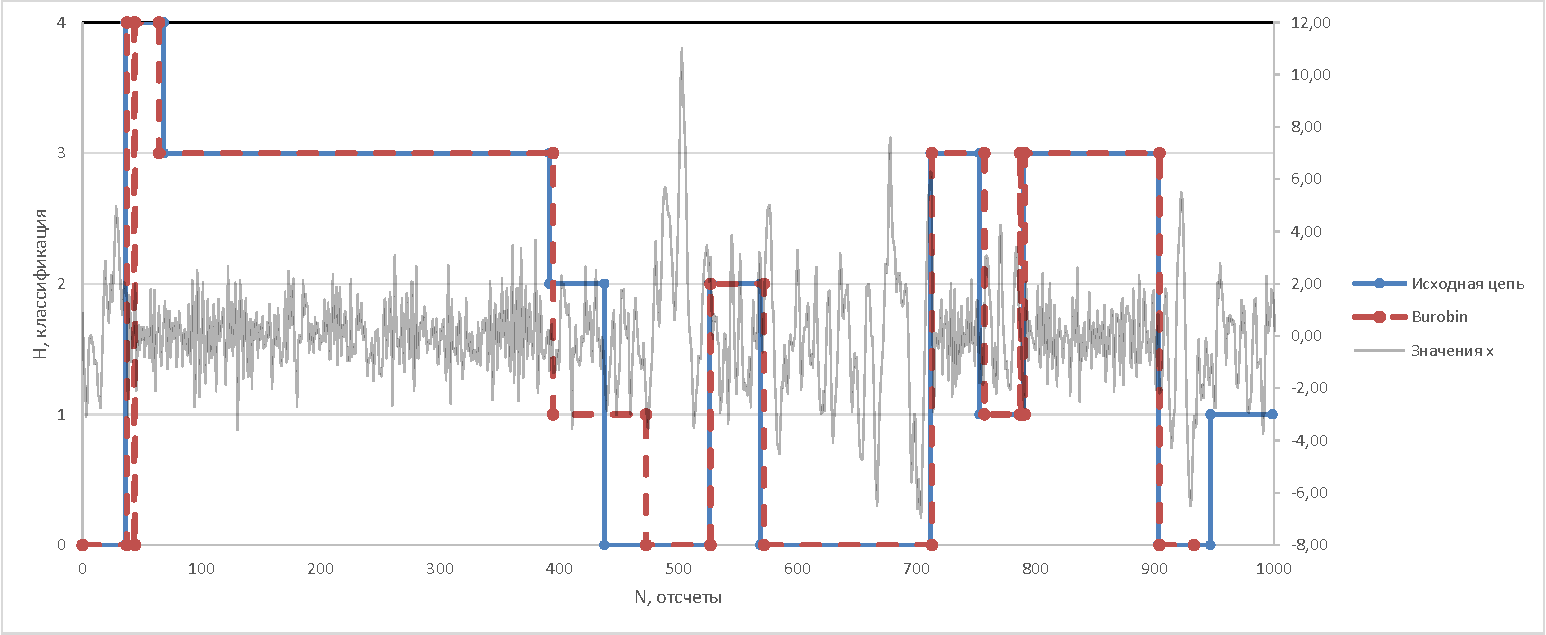
\includegraphics[width=\linewidth]{1k_burobin}
\caption{Сигнал 1, t = 1000}
\end{minipage}
\begin{minipage}[h]{0.49\linewidth}
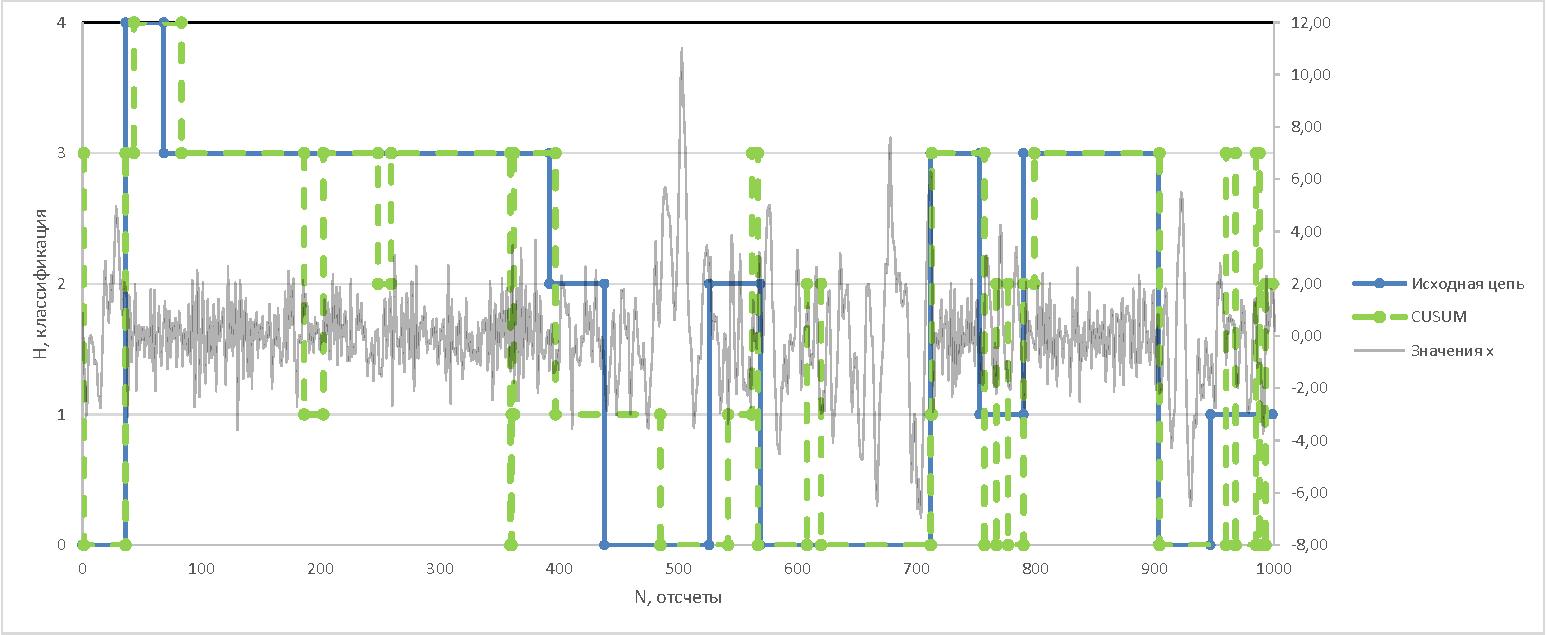
\includegraphics[width=\linewidth]{1k_cusum}
\caption{Сигнал 1, t = 1000}
\end{minipage}
\end{figure}
\end{frame}

\begin{frame}\frametitle{Результаты}
\framesubtitle{Модельный сигнал}
\begin{figure}[h]
\begin{minipage}[h]{0.4\linewidth}
\begin{table}[h]
\caption{Параметры модельного сигнала}
\label{signal_param}
\begin{tabular}{|c|c|c|c|c|}
\hline
h & $\phi_0$ & $\phi_1$ & $\phi_2$ & $B$\\
\hline
0 & 0 & 1.36 & -0.49 & 1\\
\hline
1 & 0 & 1.02 & -0.40 & 1\\
\hline
2 & 0 & 0.82 & -0.49 & 1\\
\hline
3 & 0 & 0 & -0.49 & 1\\
\hline
4 & 0 & -0.82 & -0.49 & 1\\
\hline
\multicolumn{5}{|c|}{$q_{ii} = 0.99$}\\
\hline
\multicolumn{5}{|c|}{$q_{ij} = 0.0025$, $i \neq j$}\\
\hline
\end{tabular}
\end{table}
\end{minipage}
\begin{minipage}[h]{0.4\linewidth}
Было проведено исследование качества обоих алгоритмов. В качестве меры точности алгоритма было взято среднее время совпадения построенной сегментации с оригинальной, усредненное по $N = 20000$ запусков. Были получены следующие результаты:
\end{minipage}
\end{figure}
$$t = 1000,\; Q_B = 0.86795,\; Q_{CUSUM} = 0.76240$$
$$t = 2000,\; Q_B = 0.86408,\; Q_{CUSUM} = 0.75599$$
$$t = 3000,\; Q_B = 0.86235,\; Q_{CUSUM} = 0.75323$$
\end{frame}

\begin{frame}\frametitle{Результаты}
\framesubtitle{Сигнал с вентилятора}
Были произведены 3 записи шума вентилятора в нормальном режиме работы и с разладкой(в работающий вентилятор засовывалась бумажка) в формате [норма|разладка|норма] по 20 секунд на каждый сегмент. Из каждой сегмента записи было вырезано по секундному отрезку и составлены сигналы длиной по 3 секунды. Общее количество отсчетов в каждом сигнале составило $3$с $\cdot\;44100$Гц $ = 132300.$
\begin{figure}[h]
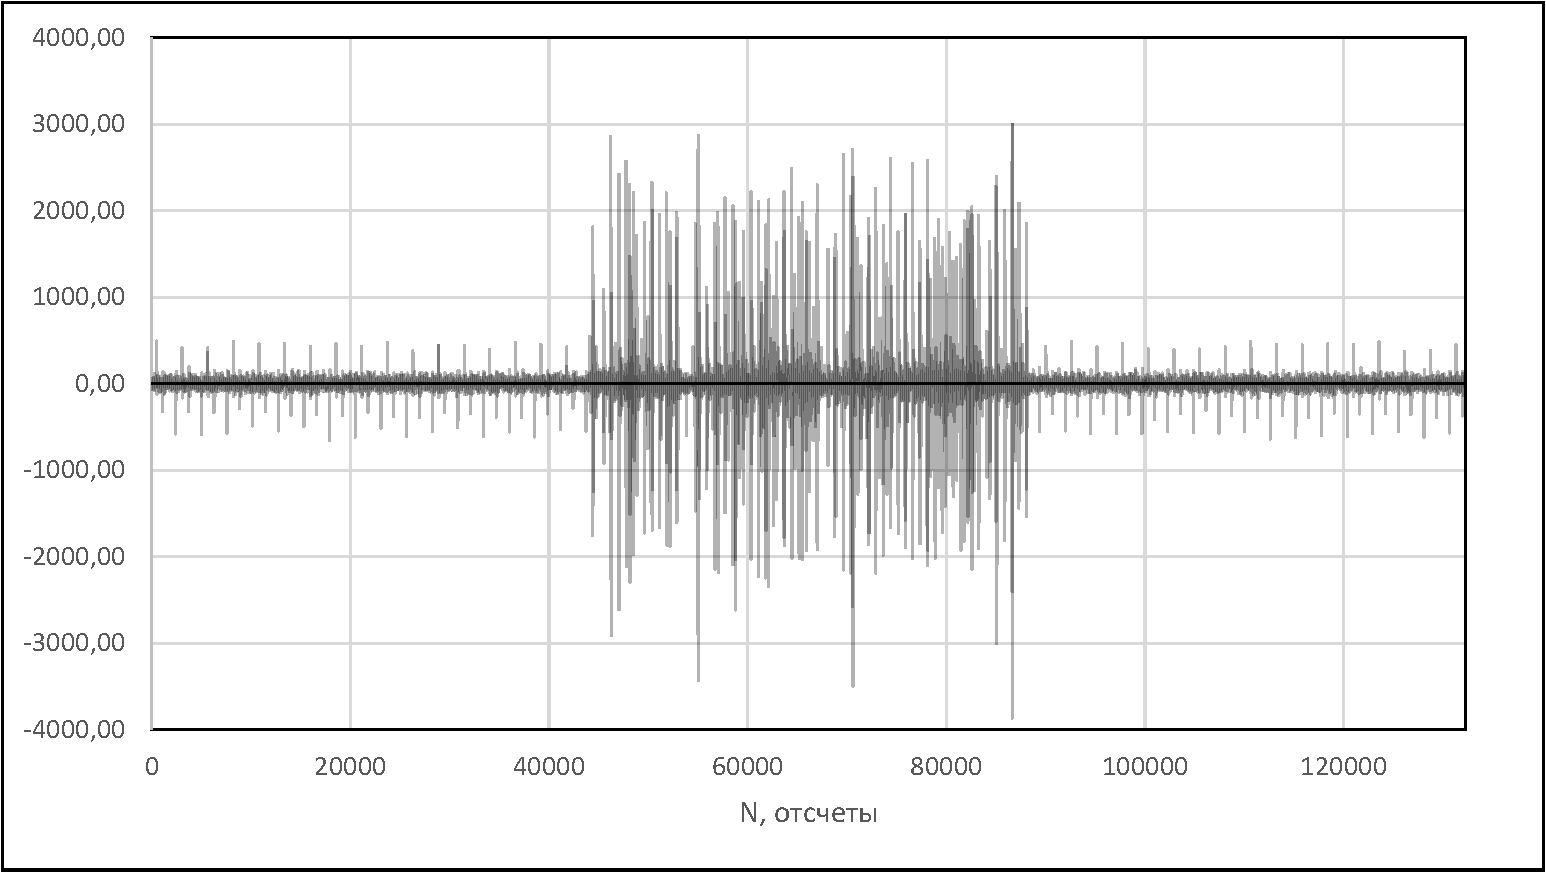
\includegraphics[width=0.7\linewidth]{signal_example}
\caption{Пример анализируемого сигнала}
\end{figure}
\end{frame}

\begin{frame}\frametitle{Результаты}
\framesubtitle{Сигнал с вентилятора}
Один из сигналов был использован для подбора параметров для алгоритмов. С помощью МНК были определены коэффициенты авторегрессии с глубиной модели $P = 10$. На графиках показаны зависимости коэффициентов авторегрессии для этого сигнала а) до разладки, б) во время разладки от количества отсчетов, анализируемых МНК. 
\begin{figure}[h]
\begin{minipage}[h]{0.49\linewidth}
\center{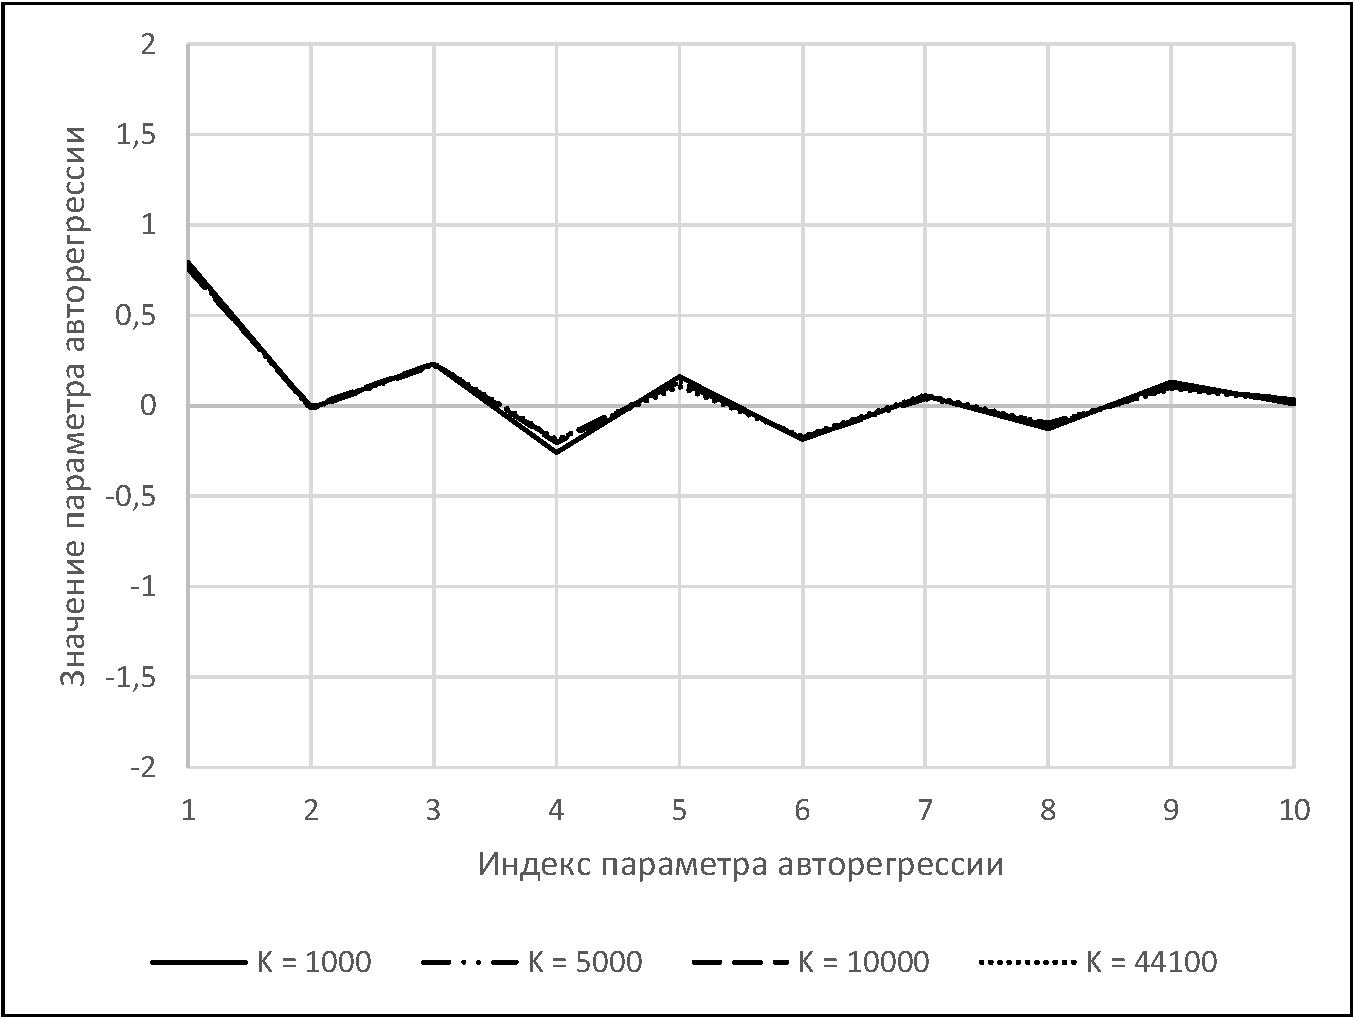
\includegraphics[width=\linewidth]{autoregression_params_normal} \\а)}
\end{minipage}
\begin{minipage}[h]{0.49\linewidth}
\center{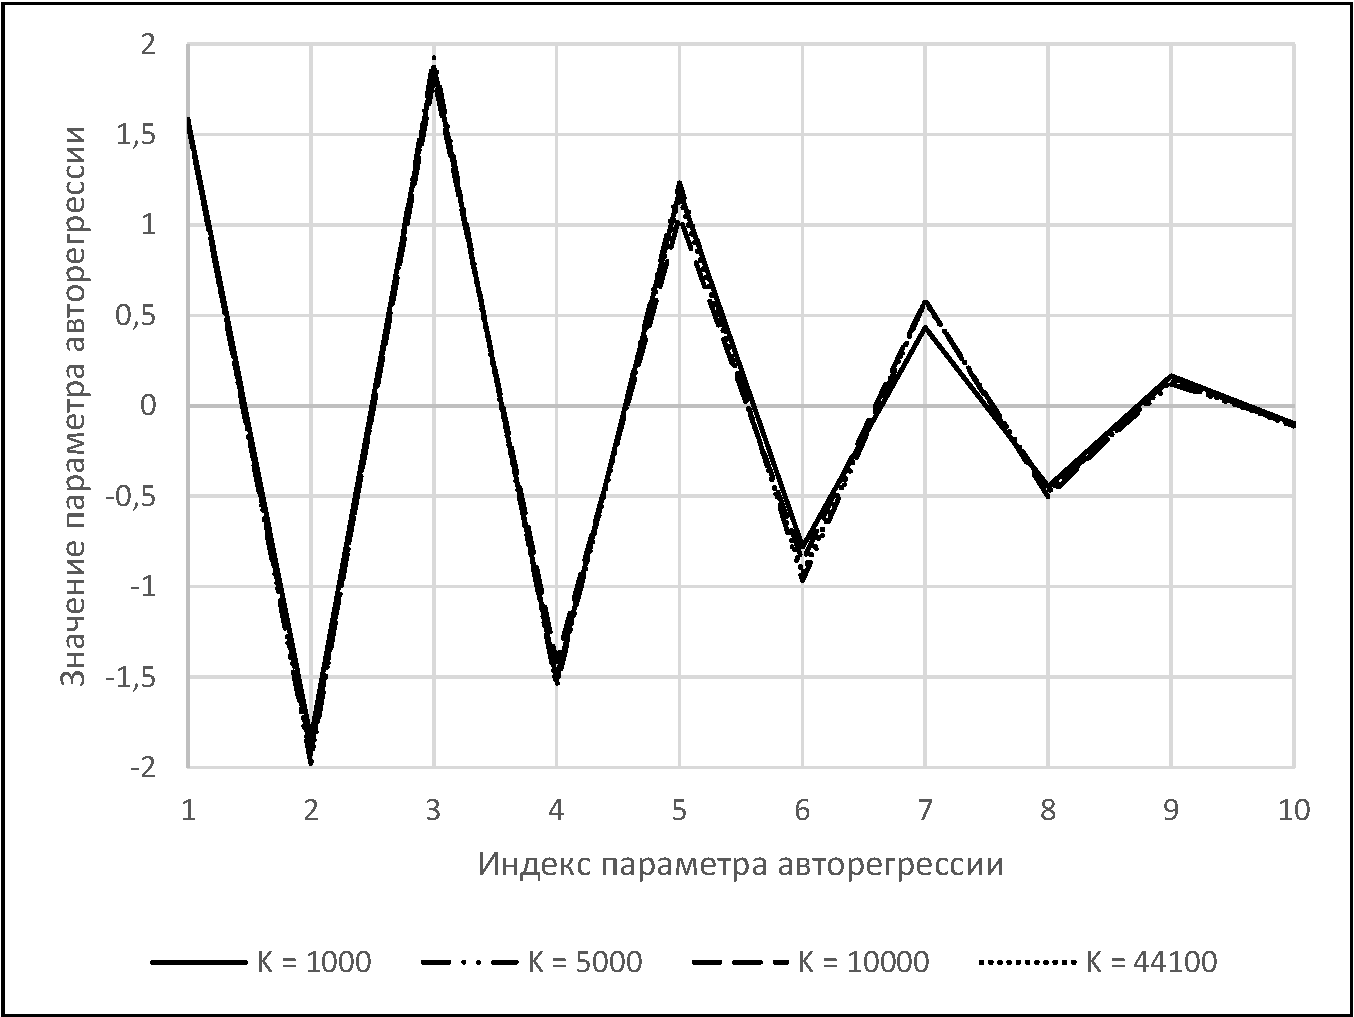
\includegraphics[width=\linewidth]{autoregression_params_disaster} \\б)}
\end{minipage}
\caption{Значения коэффициентов авторегрессии до и во время разладки}
\end{figure}
\end{frame}

\begin{frame}\frametitle{Результаты}
\framesubtitle{Сигнал с вентилятора}

\begin{table}[h]
\caption{Оценки коэффициентов авторегрессий, полученные МНК}
\begin{tabular}{|c|c|c|c|c|c|c|c|c|c|c|c|c|}
\hline
h & $\phi_0$ & $\phi_1$ & $\phi_2$ & $\phi_3$ & $\phi_4$ & $\phi_5$ & $\phi_6$ & $\phi_7$ & $\phi_8$ & $\phi_9$ & $\phi_{10}$\\
\hline
0 & 0 & 0.78 & 0 & 0.23 & -0.19 & 0.11 & -0.17 & 0.06 & -0.1 & 0.1 & 0\\
\hline
1 & 0 & 1.58 & -1.94 & 1.88 & -1.53 & 1.16 & -0.93 & 0.58 & -0.47 & 0.14 & -0.11\\
\hline
\end{tabular}
\end{table}

В таблице $h_0$ соответствует нормальной работе вентилятора, а $h_1$ - разладке. Подобранные параметры для алгоритмов составили \center{$B(h_i) = 10^5,\; q_{ii} = 0.99999,\; T_{ij} = 4 \cdot 10^6.$}
\begin{figure}[h]
\begin{minipage}[h]{0.49\linewidth}
\center{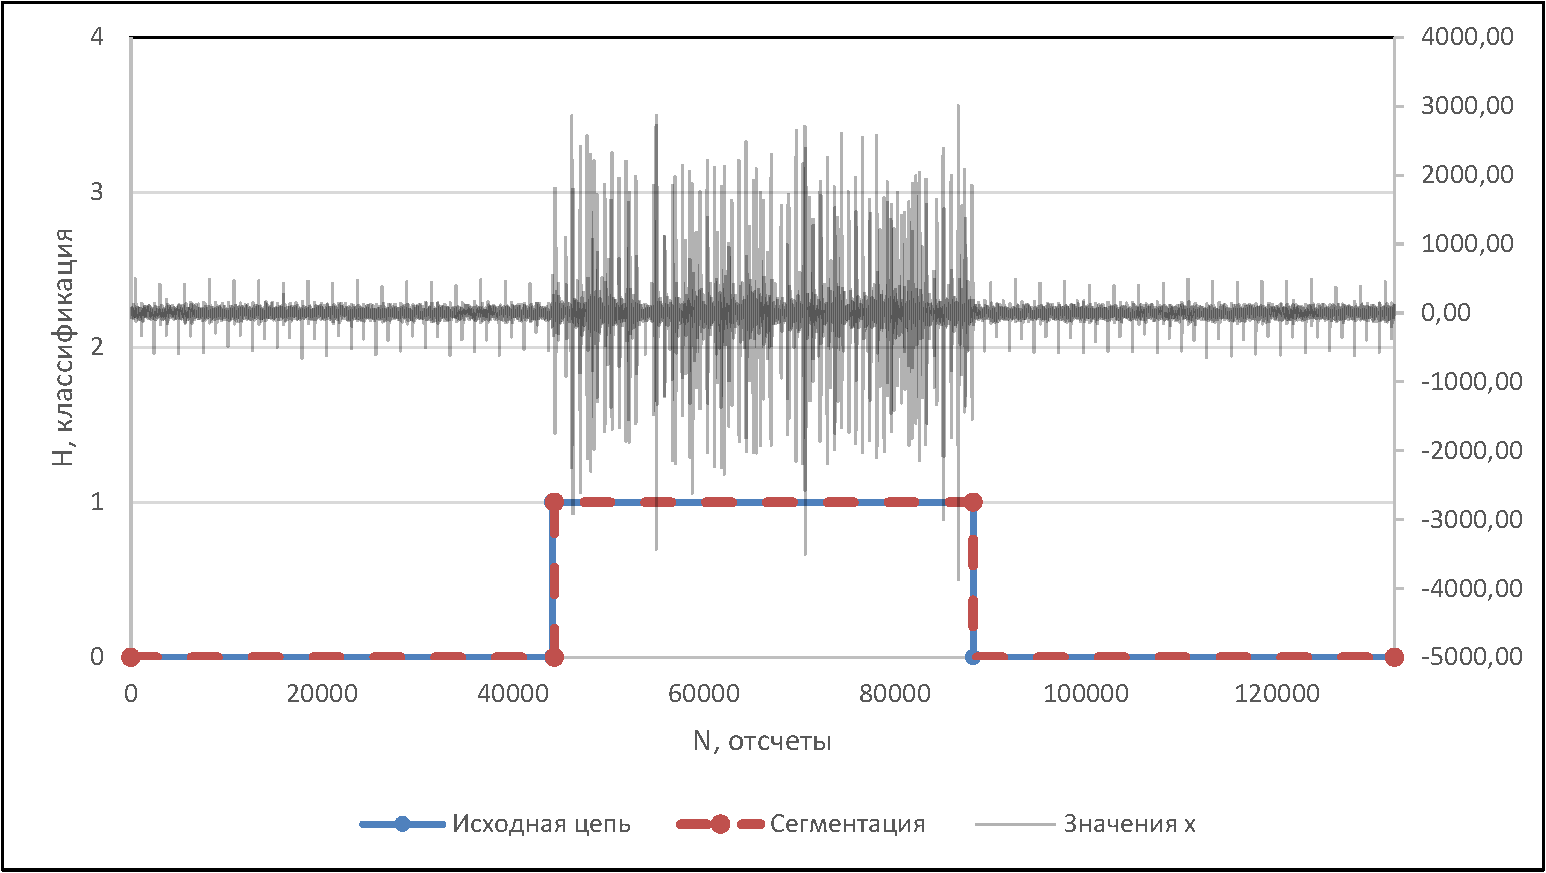
\includegraphics[width=\linewidth]{signal_cropped_1_burobin} \\а) алгоритм Буробина}
\end{minipage}
\begin{minipage}[h]{0.49\linewidth}
\center{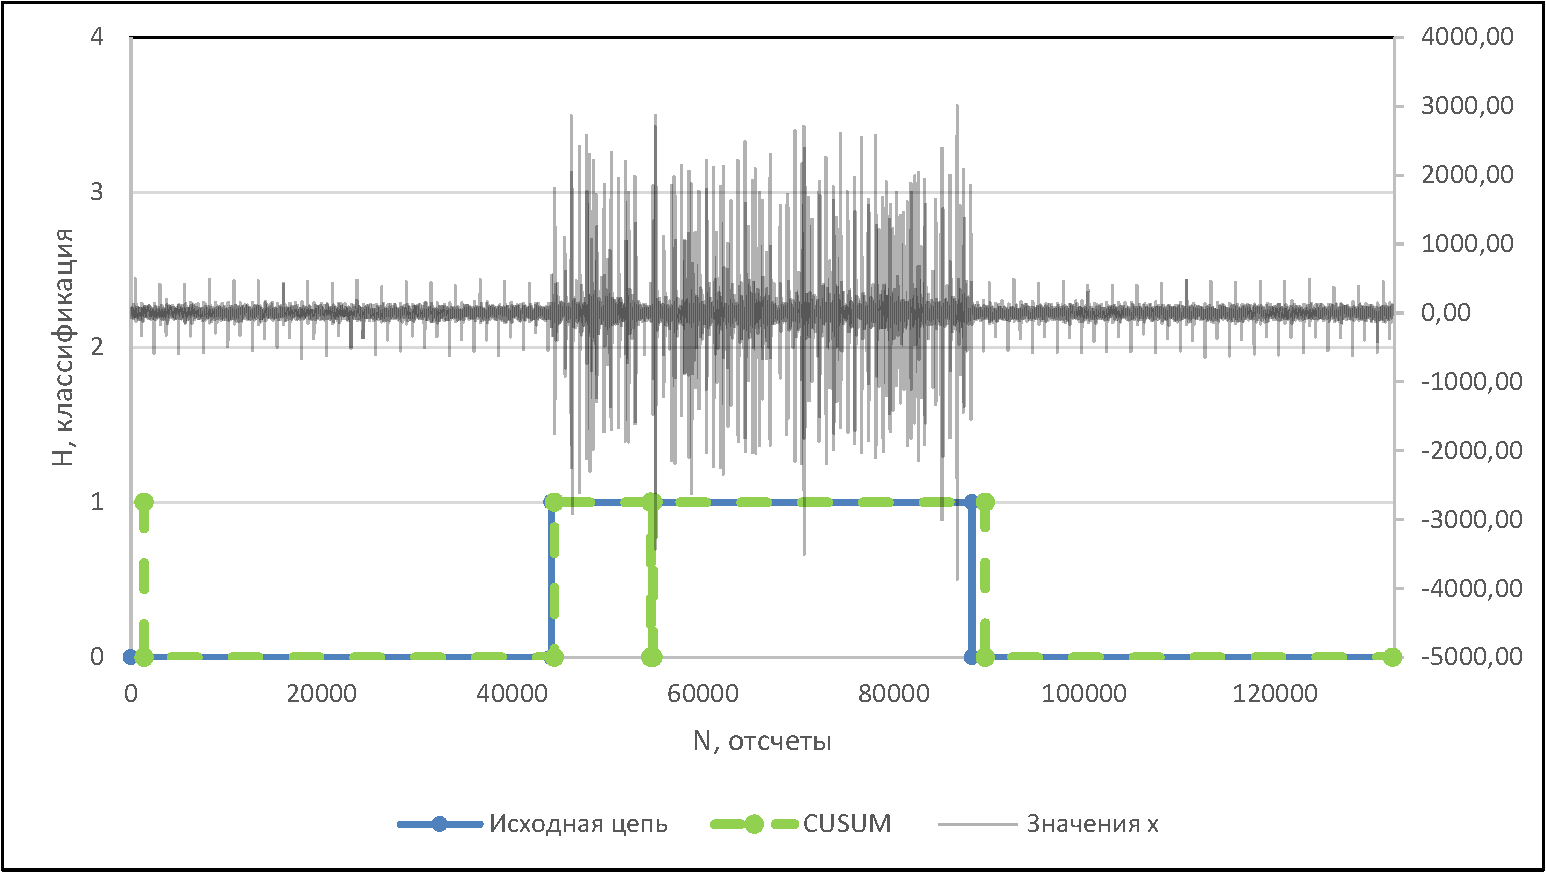
\includegraphics[width=\linewidth]{signal_cropped_1_cusum} \\б) CUSUM}
\end{minipage}
\caption{Сегментация первого сигнала с вентилятора обоими алгоритмами}
\end{figure}
\end{frame}

\begin{frame}\frametitle{Результаты}
\framesubtitle{Сигнал с вентилятора}
Найденные для сигнала 1 параметры были использованы для сегментации сигналов 2 и 3:
\begin{figure}[h]
\begin{minipage}[h]{0.49\linewidth}
\center{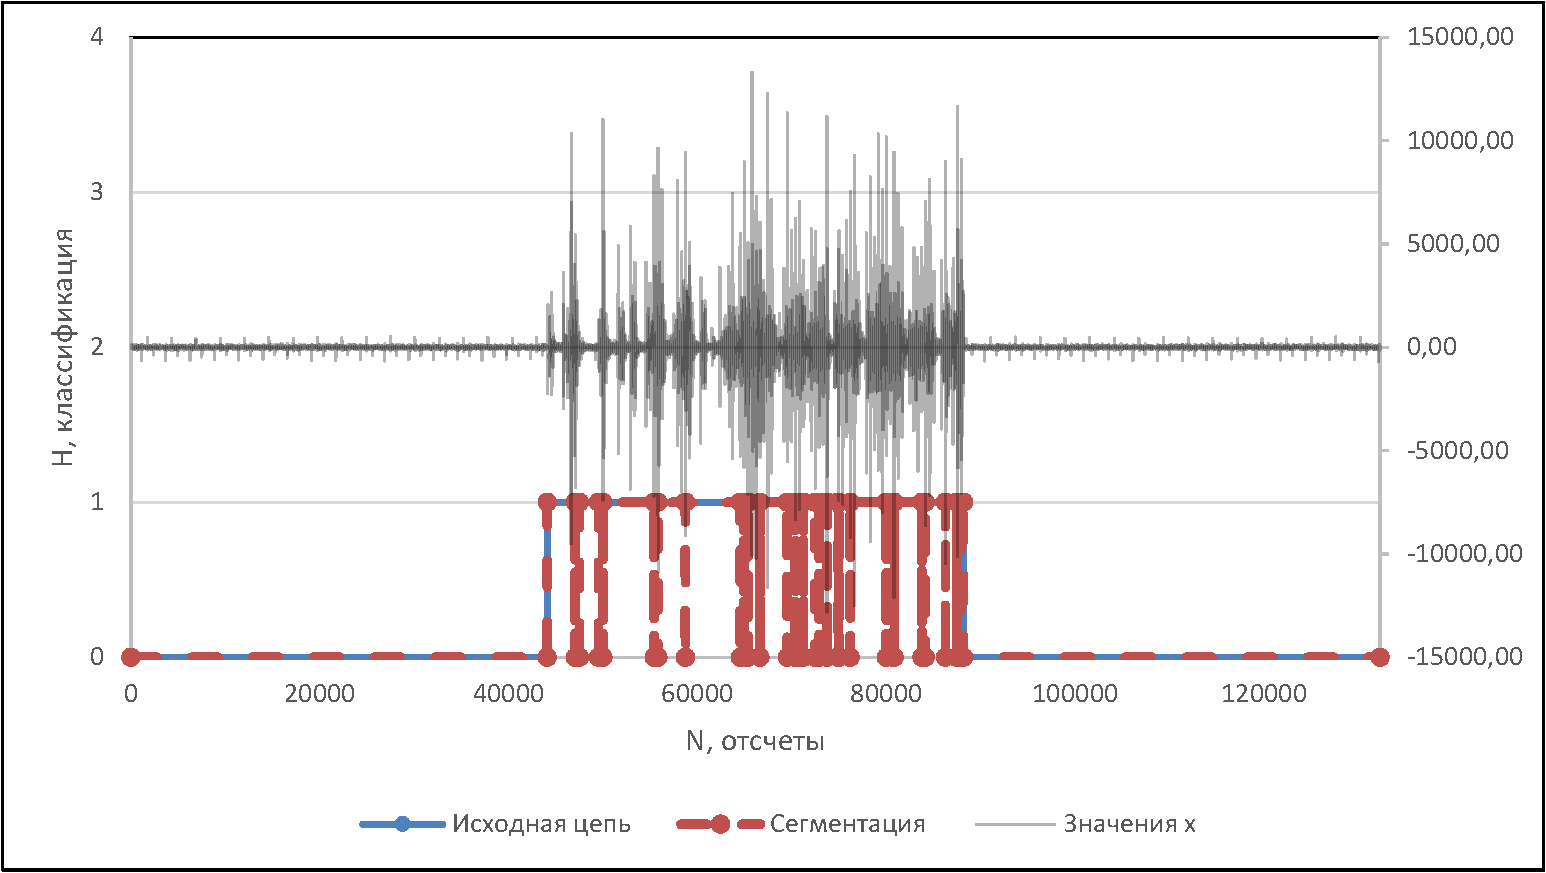
\includegraphics[width=\linewidth]{signal_cropped_2_burobin} \\а) алгоритм Буробина}
\end{minipage}
\begin{minipage}[h]{0.49\linewidth}
\center{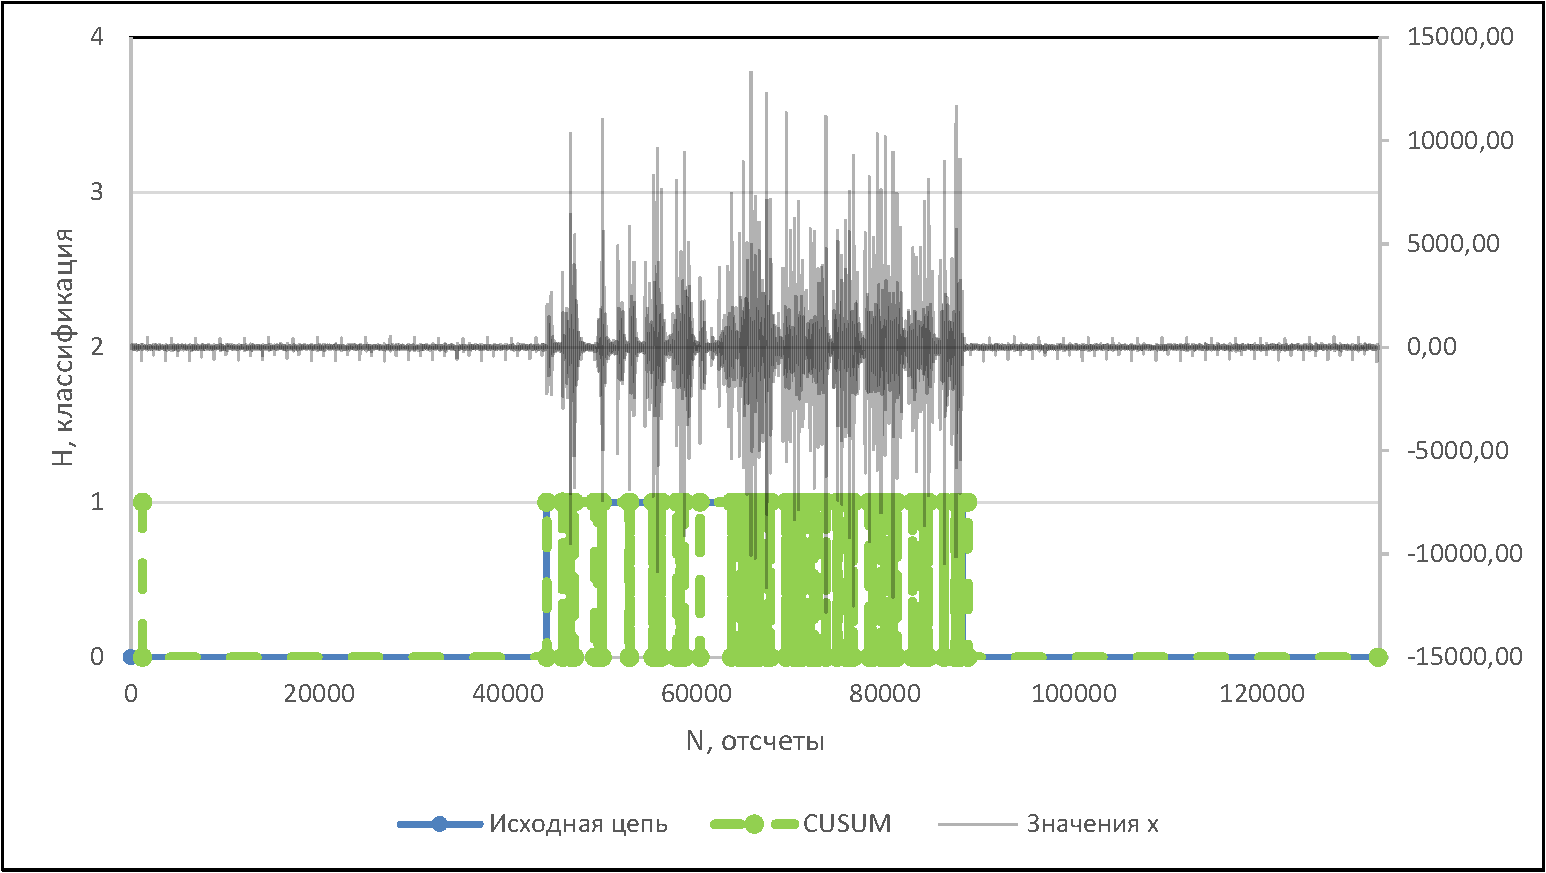
\includegraphics[width=\linewidth]{signal_cropped_2_cusum} \\б) CUSUM}
\end{minipage}
\caption{Сегментация сигнала 2}
\end{figure}
\end{frame}

\begin{frame}\frametitle{Результаты}
\framesubtitle{Сигнал с вентилятора}

\begin{figure}[h]
\begin{minipage}[h]{0.49\linewidth}
\center{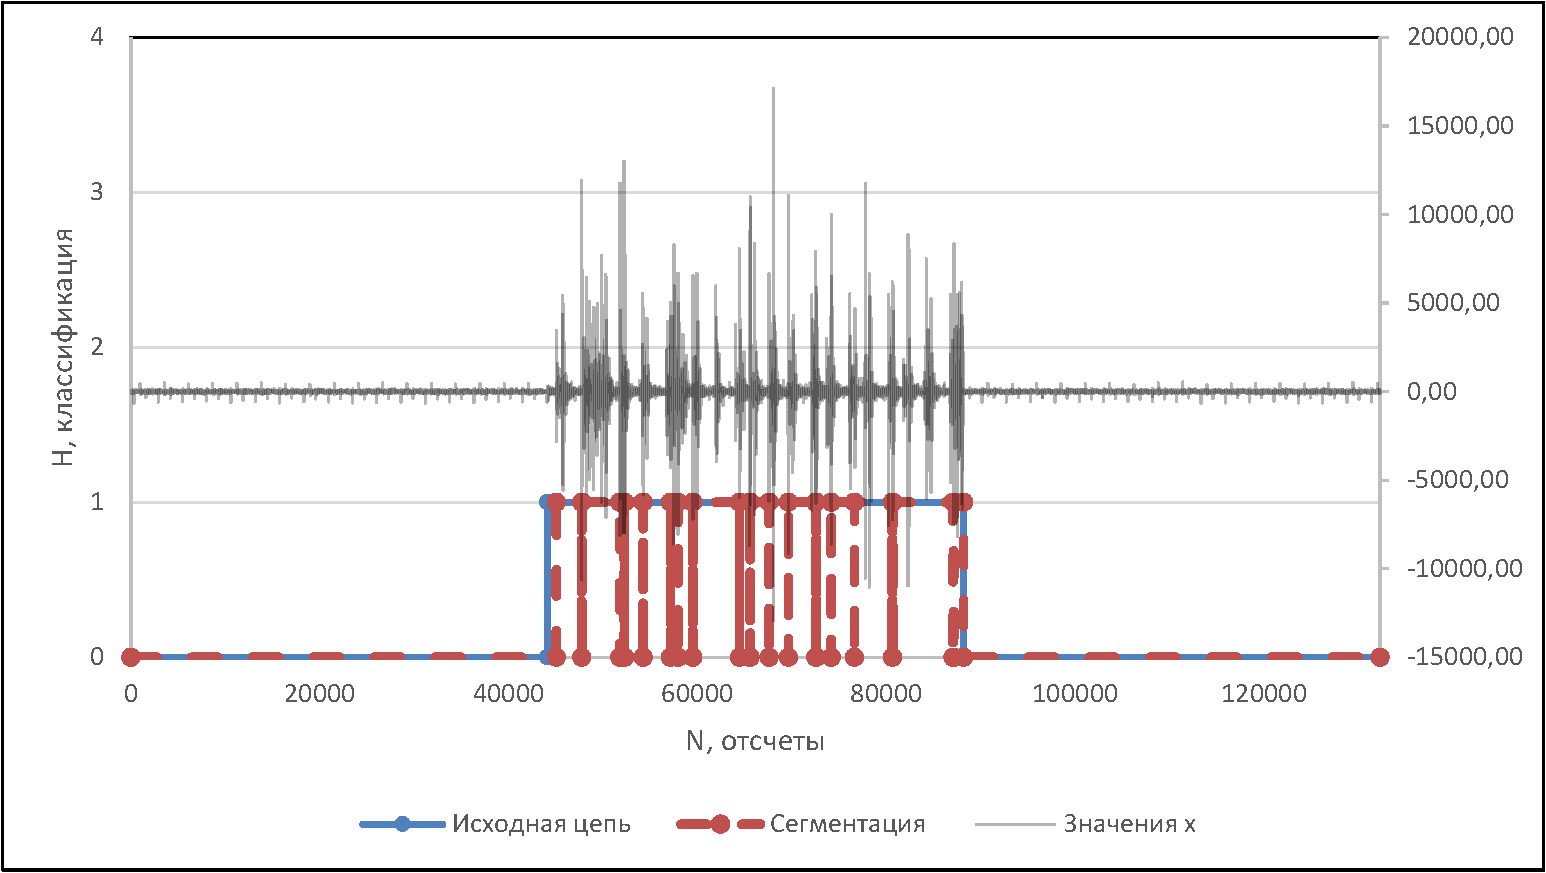
\includegraphics[width=\linewidth]{signal_cropped_3_burobin} \\а) алгоритм Буробина}
\end{minipage}
\begin{minipage}[h]{0.49\linewidth}
\center{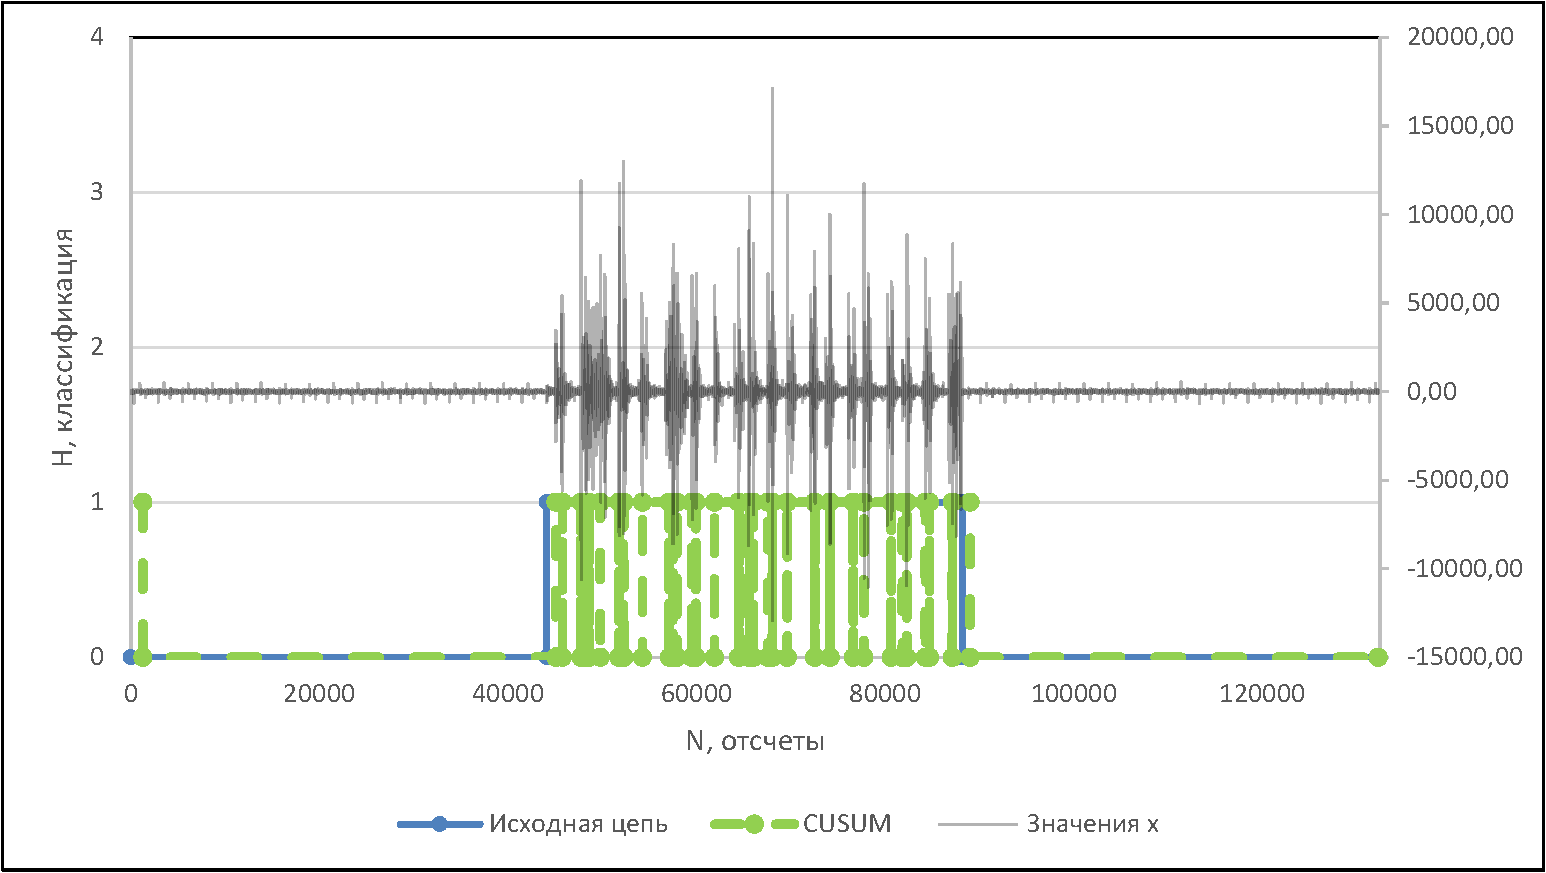
\includegraphics[width=\linewidth]{signal_cropped_3_cusum} \\б) CUSUM}
\end{minipage}
\caption{Сегментация сигнала 3}
\end{figure}
\end{frame}

\begin{frame}\frametitle{Выводы}
Результаты, полученные из экспериментов с модельным сигналом показывают, что
\begin{itemize}
\item Алгоритм на основе метода динамического программирования
\begin{itemize}
\item имеет в среднем на 10\% большую точность по сравнению с алгоритмом
на основе статистики CUSUM
\item учитывает вероятности переходов, заданные в матрице $Q$
\end{itemize}
\item Алгоритм на основе статистики CUSUM:
\begin{itemize}
\item качество сегментации сильно зависит от выбора пороговых
значений $T_{ij}$ для каждой пары переходов
\item легче в реализации
\item более производителен
\end{itemize}
\end{itemize}

Эксперименты на реальном сигнале с электромеханического
устройства (вентилятора) показали, что рассматриваемый
подход применим к реальным сигналам, однако требует некоторой доработки.
\end{frame}

\begin{frame}\frametitle{Список литературы}
\begin{thebibliography}{99}
\bibitem{TVAR} Chukiet Sodsri, ``Time-varying autoregressive modelling for nonstationary acoustic signal and its frequency analysis'', 2003
\bibitem{vehicles} Kie B. Eom, ``Analysis of Acoustic Signatures from Moving Vehicles Using Time-Varying Autoregressive Models'', Multidimensional Systems and Signal Processing 10, pp. 357-378, 1999
\bibitem{bio} Akay, Y.M., ``Noninvasive acoustical detection of coronary artery disease: a comparative study of signal processing methods'', Biomedical Engineering 40, pp. 571-578, 1993
\bibitem{burobin} Николай Буробин, Вадим Моттль, Илья Мучник, ``Алгоритм определения моментов многократного изменения свойств случайного процесса на основе метода динамического программирования'', Статистические проблемы управления 65, стр. 49-57, 1984.
\bibitem{nikiforov} Mich\`{e}le Basseville, Igor V. Nikiforov, ``Detection of Abrupt Changes: Theory and Application'', pp. 35-43, 1998
\end{thebibliography}
\end{frame}
\end{document}